\section{Enigma und Turing Bombe}
In diesem Abschnitt wird die Enigma und ihre Entschlüsselung Thematisiert. Des weiteren wird auf die Historischen Hintergründe eingegangen, auf ihre Funktionsweise sowie ihre Fehler.

\subsection{Enigma}
Die Enigma Maschine ist eine Verschlüsselungsmaschine, die im zweiten Weltkrieg von den Deutschen genutzt wurde um militärische Fernkommunikation zwischen ihren Truppen zu etablieren. Diese sollte ihnen mit unter einen Entschiedenen Vorteil liefern. Dennoch hatte diese Verschlüsselung eine paar sehr große Probleme, die dazu Führten, dass die Alliierten immer wieder sehr viele Kommunikation entschlüsseln konnten.\\
Hauptbestandteile der Enigma waren:
\begin{enumerate}
\item Eingabetastatur
\item Lichtanzeige
\item Steckbrett
\item Reflektor
\item drei Zahnräder
\end{enumerate}

\subsubsection{Eingabetastatur}
Eine Schreibmaschinen ähnliche Tastatur mit allen 26 Buchstaben des Alphabets, in die man die Nachricht eintippen konnte. Diese Tastatur war mit dem Steckbrett verknüpft.

\subsubsection{Lichtanzeige}
Eine Anzeige mit allen 26 Buchstaben des Alphabets, die einzeln beleuchtet werden und die verschlüsselte Nachricht anzeigen z.B ein H wird eingetippt und ein R wird beleuchtet.

\subsubsection{Steckbrett}
\label{sec:steck}
Das Steckbrett, welches hinten an der Enigma Maschine angebracht war, diente zur weiteren Verschlüsselung, da man hier bis zu 13 von 26 Buchstaben manuell miteinander verlinken konnte. Somit wurde z.B. ein eingegebenes A zu einem H und vice versa. Wenn kein Kabel eingesteckt wurde, dann wurde der Buchstabe einfach normal durch geschallten. Meist wurden nur 10 umgesteckt.

\subsubsection{Zahnräder}
\label{sec:rader}
Die Zahnräder dienten zum weiteren Verschlüsseln der Nachrichten und jedes Zahnrad hatte 26 Stufen für jeden Buchstaben des Alphabets. Wobei das Signal nun innerhalb des Rades durch neue Verkabelung auf einen anderen Buchstaben geleitet wurde. Das Signal wurde an das nächste Rad weiter geleitet, dort passiert das selbe nochmal. Es gab 8 verschiedene Arten von Rädern, diese besaßen pro Art immer die Selben Verkabelung innerhalb der Zahnräder. Das Erste Zahnrad, welches die Eingabe passierte drehte sich bei jedem Tastendruck um einen Buchstaben weiter. Die Nachfolgenden Zahnräder drehten sich immer dann um eines wenn sich das vorherige an seinem Überrollpunkt befindet dieser ist meist wenn sich, dass Rad einmal um sich selber gedreht hat, dass kann etwa bei M oder aber auch Z sein. Der Überrollpunkt konnte über einen offset Markierung an den Rädern eingestellt werden. So, dass sich die neu Verkabelung um soviel stellen wie eingestellt in eine Richtung weiter gedreht wird. Diese wurden am Anfang jeder Nachricht ein mal eingestellt. Am Anfang wurden diese Starteinstellungen über die Nachricht mitgeteilt, in dem man eine deutsches Wort mit 3 Buchstaben zweimal hintereinander gesendet hat. Was sich jedoch schnell als ziemlich schlechte Idee herausstellte und somit 1938 verboten wurde.

\subsubsection{Reflektor}
Der Reflektor schickte die Signale die von den Rollen kamen und schickte sie durch eine andere Leitung an den Rollen wieder zurück. Dieser konnte nie wieder zum gleichen Buchstaben zurück sondern wurde wieder neu Verkabelt.

\subsubsection{Beispiel}

\begin{figure}[H]
\centering
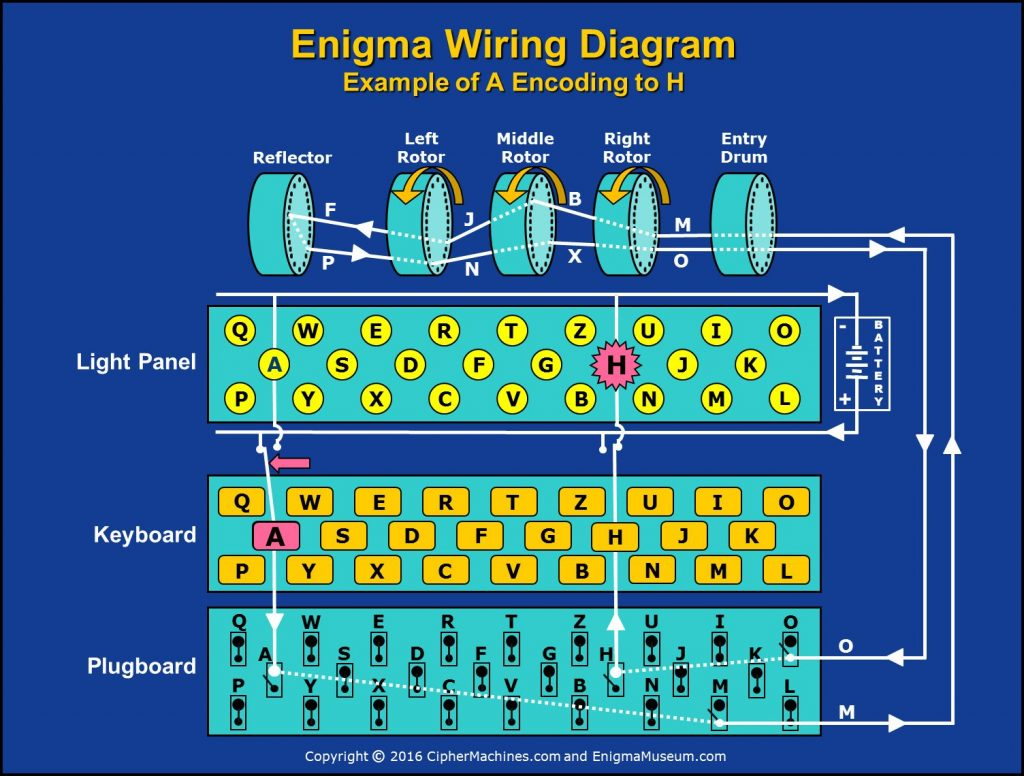
\includegraphics[scale=0.2]{Enigma_Maschine_Beispiel.jpg}
\caption{Beispiel Verkabelung}
\label{fig:enigma}
\end{figure}

Der eingegebene Buchstabe A geht erst einmal an das Steckbrett und ist hier mit dem Buchstaben M verbunden. Dieser wird dann an die Zahnräder weitergegeben, die den Buchstaben je nach Stellung verändern, hier von B zu J und schließlich F. Anschließend wird der Buchstabe wieder zurück durch die Zahnräder geleitet und kommt in diesem Beispiel als O heraus und wird wieder an das Steckbrett weitergeleitet. Der Buchstabe O ist hier mit H verbunden und so wird am Ende H in der Anzeige beleuchtet, und somit wurde A zu H verschlüsselt.

\subsection{Historie}
Turing beschäftigte sich bereits vor Beginn des zweiten Weltkriegs mit den Enigma Maschinen, allerdings waren diese von den Italienern und wesentlich simpler wie die Enigma Maschinen später genutzt von den Deutschen. Die erste version der Enigma war frei verkäuflich und wurde eher private genutzt da sie nicht viel Sicherheit bat. In dieser version gab es lediglich 3 der in Sektion \ref{sec:rader} beschriebenen Räder, die in unterschiedlicher Reihenfolge eingesetzt werden konnten. Damit gab es lediglich $3! = 6$ Anordnungsmöglichkeiten. Zu dieser Zeit gab es außerdem kein, wie in Sektion \ref{sec:steck} aufgeführtes Steckbrett. Ein polnisches Verschlüsselungsteam unter der Leitung von Marian Rejewski legte den Grundstein und knackte die Verschlüsselungen der Enigma sehr schnell dort wurden sie zum ersten mal mit Steckbrett Versionen konfrontiert. Diese knackten sie von Hand mit Hilfe von Lochpapieren. Deutschland wollte sich diese Verschlüsselungsmaschinen nun für Militärische Zwecke zu nutzen machen, so entwickelten sie die nächste Version, die militärische Enigma. In dieser version wurden zwei Zahnräder zur Auswahl hinzugefügt. Nun wurden also 3 aus 5 Zahnrädern genommen und in unterschiedlichen Anordnungen in der Enigma kombiniert. Diese wurden nachher Großflächig für die deutsche Luftwaffe und Arme eingesetzt. Doch Marine war das nicht genug. Unter Admiral Karl Dönitz wurde eine Enigma Speziell für die Marine entwickelt bei der zu erst 3 aus 8 Zahnrädern und später dann 4 aus 8 Zahnrädern für die Verschlüsselung verwendet. Zu allem Überfluss drehten sich die Räder 6 bis 8 zweimal. Damit explodierten die Möglichen Kombinationen fast exponentiell. Bei Ausbruch des Krieges wurde Turing zusammen mit Neuntausend anderen Spezialisten in den Bletchley Park geholt. Dieser Park wurde zu einer wahren Entschlüsselungsfabrik, in dem später mit Hilfe der \emph{Bombe} 39 Tausend Enigma Nachrichten im Monat entschlüsselt wurden. Die sogenannte \emph{Bombe} war eine automatisierte Maschine zur Entschlüsselung der Enigma Nachrichten. Diese wurde ursprünglich von den Polen bis zur Invasion entwickelt. Durch die Invasion jedoch Übergaben sie die von den Polen \emph{Bomba} genannte Maschine an die Briten. Dort bauten sie die Maschine weiter aus und bauten im Zuge des Krieges zwischen 60 und 100 verschiedene \emph{Bombes} in Großbritannien und noch einmal mindestens so viel in der USA. Dort halfen sie dem Briten beim dechiffrieren per Unterseekabel. In Bletchley Park wurde der Platz sehr eng deswegen wurden um das eigentliche Gebäude mehrere Hütten gebaut die sogenannten \emph{Huts}. Schnell bekamen die \emph{Huts} spezielle aufgaben. So war Hut 8, der Arbeitsplatz von Turing, mit der Entschlüsselung der sehr schweren Marine Enigma betraut. Während die normale Enigma Texte der Armee und der Luftwaffe in Hut 6 unter der Leitung von Gordon Welchman, ein weiterer berühmter Statistiker, bearbeitet wurden.  \cite{enigmaproblem1} \cite{theessentialturing}

\subsection{Schwachstellen}
Die Enigma hatte einige Schwachstellen, die im ersten Moment vielleicht nicht als solche erscheinen. Dazu gehörte ein mal, dass der Reflektor die Signale nie auf den gleichen Buchstaben zurück leiten konnte. Dadurch konnte man versuchen bekannte Wörter wie zum Beispiel "Wetterbericht" über den verschlüsselten Text halten. Wenn eine der Buchstaben in dem Wort mit dem verschlüsselten Text an der Stelle übereinstimmte dann konnte es sich nicht um das Wort handeln. Ziel der Entschlüsselung war es heraus zu finden mit welchen der Räder und mit welchen Radeinstellungen sie die \emph{Bombe} bestücken mussten. Diese sollte dann den Rest tun. Des weiteren war bei den Rollen 6 bis 8 der Marine das zweite überrollen ein Indikator dafür das ein solches Rad eingesetzt wurde. Dies konnte die Möglichkeiten sehr einschränken. Das oben genannte Problem mit dem doppelt senden eines deutschen Wortes mit 3 Buchstaben hat natürlich dafür gesorgt, dass hier über die Wahrscheinlichkeiten in der Sprache es sehr einfach war die Ring Einstellung zu erraten. Mit Hilfe des oben genannten Reflektor Problems minimierte es natürlich weiter die Möglichkeiten. Dieses Problem bemerkten die Deutschen und verbaten diese Übersendung von Ringeinstellungen. Des weiteren Halfen gestohlene Codebücher und Insider Informationen beim Entschlüsseln. Des weiteren halfen natürlich die morgendlichen um Punkt 6 Uhr gesendeten Wetterberichte, denn diese begannen mit dem Wort \emph{Wetterbricht} und endeten mit \emph{Heil Hitler}. \cite{enigmaflaw} \cite{enigmaproblem1}